\documentclass{book}
\usepackage[utf8]{inputenc}

\usepackage{graphicx}
\title{Computational Neuroscience}
\author{Huynh Xuan Phung - Coursera}
\date{ }
\usepackage{color}   %May be necessary if you want to color links
\usepackage{hyperref}
\hypersetup{
    colorlinks=true, %set true if you want colored links
    linktoc=all,     %set to all if you want both sections and subsections linked
    linkcolor=blue,  %choose some color if you want links to stand out
} 
\begin{document}
 
\maketitle
 
\tableofcontents

\chapter{Introduction and Basic Neurobiology}

\section{Computational Neuroscience}
\subsection{Descriptive Models}

What is Computational Neuroscience?
Computational Neuro-science provides tools and methods for "characterizing what nervous systems do, determining how they function, and understanding why they operate in particular ways"

Descriptive Models (What)

Mechanistic Models (How)

Interpretive Models (Why)

Frequency of spikes = f(Light bar's orientation). 

"receptive field" of a neuron is the particular orientation of a bar of light that produces the best response. That is maximizes f(Light Bar's orientation) (45 degree is maximize).

A greater response corresponds to more frequent "spikes" (or action potentials)

Receptive Field: is specific properties of a sensory stimulus that generate a strong response from the cell

Examples:
\begin{itemize}
	\item {Spot of light that turns on at a particular location on the retina}
	\item{Bar of light that turns on at a particular orientation and location on the retina}
\end{itemize} 

\subsection{Descriptive Model of Receptive Fields}
\begin{figure}[h]
\centering
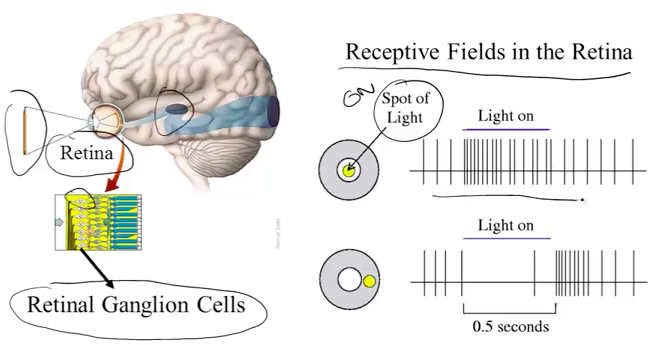
\includegraphics[width=0.7\linewidth]{figures/ReceptiveField_Retina}
\caption{}
\label{fig:receptivefieldretina}
\end{figure}

Center-Surround Receptive Fields on the Retina

--- On-Center Off-Surround: center of the small patch of retina associated with the cell

The ON-Center/ Off-Surround receptive field can be thought of as a filter. The filter causes activation with stimuli concentrates on the center of the receptive field and depressing activation with stimuli which are concentrated in the surround.

\subsection{Descriptive models: Cortical Receptive Fields}
\begin{figure}[h]
\centering
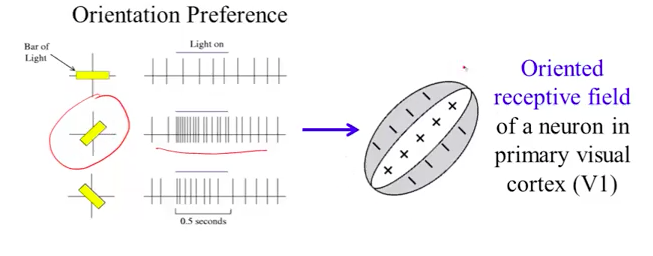
\includegraphics[width=0.7\linewidth]{figures/ReceptiveField_V1}
\caption{}
\label{fig:receptivefieldv1}
\end{figure}

Oriented receptive field of a neuron in primary visual cortex (V1)



\subsection{Mechanistic and Interpretive Models}

Mechanistic Model of Receptive File

\begin{figure}[h]
\centering
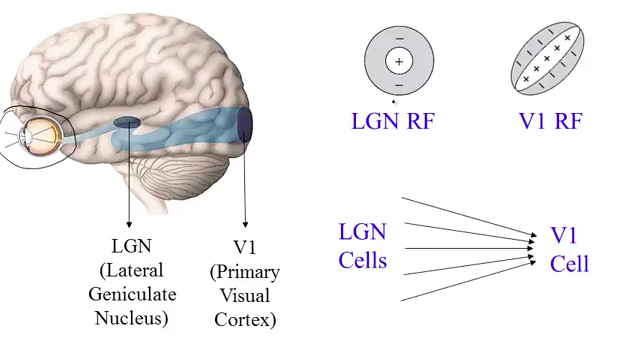
\includegraphics[width=0.7\linewidth]{figures/mechanistic_v1}
\caption{}
\label{fig:mechanisticv1}
\end{figure}

Number of LGN cells converges to one V1 cell: arrange LGN to one V1 cell

\begin{figure}[h]
\centering
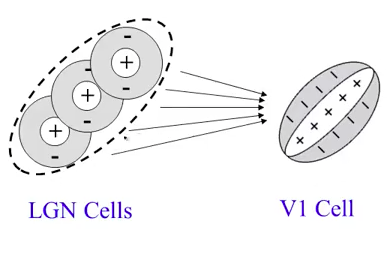
\includegraphics[width=0.7\linewidth]{figures/V1Cell}
\caption{}
\label{fig:v1cell}
\end{figure}

\subsection{Interpretive Model of Receptive Fields}

Why do they have orientation, or selected of black and white dot?

Efficient Coding Hypothesis: Suppose the goal is to represent images as faithfully ans efficiently as possible using neurons with receptive fields $RF_1,RF_2$, etc 

Given image I, we can reconstruct I using neural response $r_1,r_2$ ..

$ \hat{I} = \sum_{i} RF_i r_i$

Idea: What are the $RF_i$ that minimize the total squared pixelwise errors between I and $\hat{I}$ and are as independent as possible?


Start out with random $RF_i$, and run your efficient coding algorithm on natural image patches. efficient coding: Sparse coding/ ICA/ Predictive coding.



\section{The Electrical Personality of Neurons}
Neuronal Zoo

-- Visual cortex, Cerebellum, Optic Tectum

Neron Doctrine: 

The brain is broken into individual, discrete parts called neurons

The shape of neuron varies in some general way form one area of the brain to another

Dendrites are the inputs ends of the neuron, whereas axons are the outputs ends.

\begin{figure}[h]
\centering
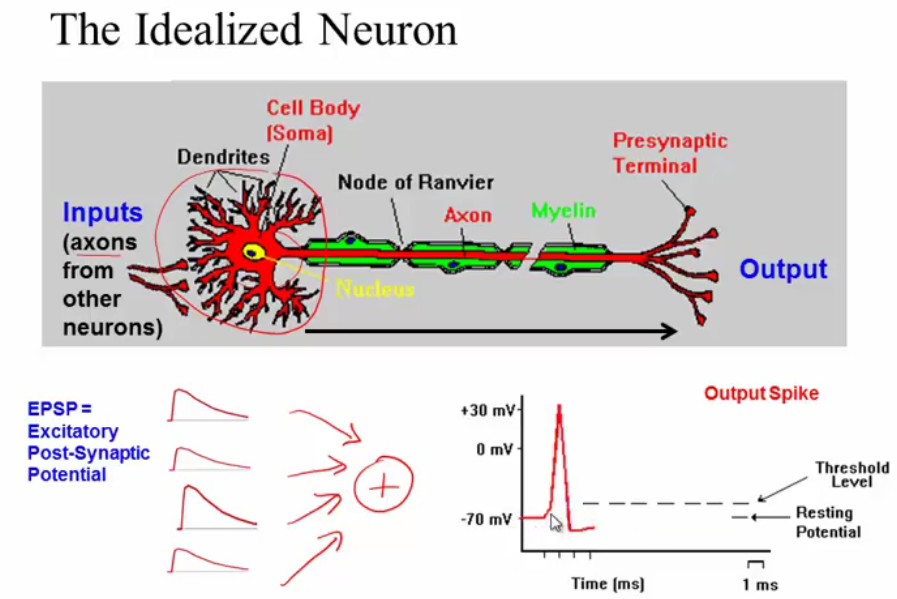
\includegraphics[width=0.7\linewidth]{./figures/neuron}
\caption{Spikes form a neuron occur when the sum of inputs from neighboring neurons reaches a certain threshold}
\label{fig:neuron}
\end{figure}

What is a Neuron?

--- A leaky bag of charged liquid

--- Contents of the neuron enclosed within a cell membrane

--- Cell membrane is a lipid bilayers. Bilayer is impermeable to charged ion species such as $Na^+$, $Cl^-$ and $K^+$
--- --- Ionic channels embedded in membrane allow icons to flow in or out

--- Each neuron maintain a potential difference across its membrane

--- --- Inside in about -70mV relative to outside

--- --- [Na+] and [Cl-] higher outside; [K+] and organic anions [A-] higher inside

--- --- Ionic pump maintains -70mV difference by expelling Na+ out and allowing K+ in

\begin{figure}[h]
\centering
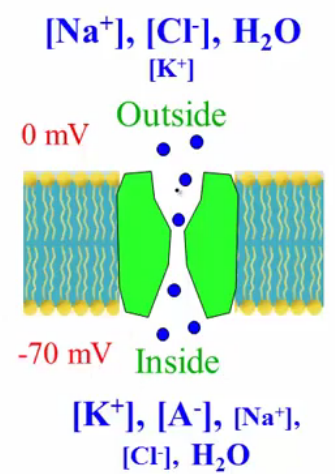
\includegraphics[width=0.7\linewidth]{./figures/ionchanel}
\caption{Neuron membrane}
\label{fig:ionchanel}
\end{figure}

Ionic Channels: the Gate-keepers

Ionic channels in membrane are proteins that are selective and allow only specific ions to pass through

Ionic channels are gated:

--- Voltage-gated: Probability of opening depends on membrane voltage

--- Chemically-gated: Binding to a chemical cause channel to open

--- Mechanically-gated: Sensitive to pressure or stretch 

Gate Channels allow Neuronal Signaling

--- Input form other neurons $\rightarrow$ chemically-gate channels (at synapses) open $\rightarrow$ Changes in local membrane potential

--- This in turn cause opening/closing of voltage-gate channels in dendrites, body, and axon, resulting in depolarization (positive change in voltage) or hyper-polarization (negative change in voltage)

Strong enough depolarization cause a spike or action potential

The Output of a Neuron: Action Potential (Spike)

Voltage-gated channels cause action potentials (spikes)

1. Strong depolarization opens Na+ channels, causing rapid Na+ influx and more channels to open until they inactivate

2. K+ outflux restores membrane potential



\begin{figure}[h]
\centering
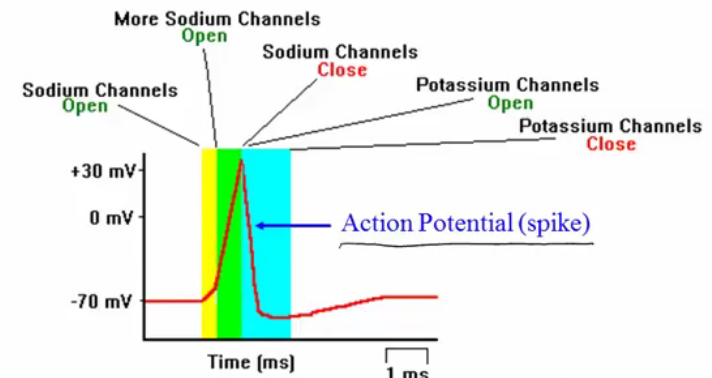
\includegraphics[width=0.7\linewidth]{./figures/spikes}
\caption{spikes time}
\label{fig:spikes}
\end{figure}


Active Wiring: Myelination of Axons

Myelin due to oligodendrocytes (glial cells) wrap axons and enable fast long-range spike communication

--- Action potential hops form one non-myelinated region (node of Ranvier) the the next (saltatory conduction)

--- Active wire allows lossless signal propagation

\begin{figure}[h]
\centering
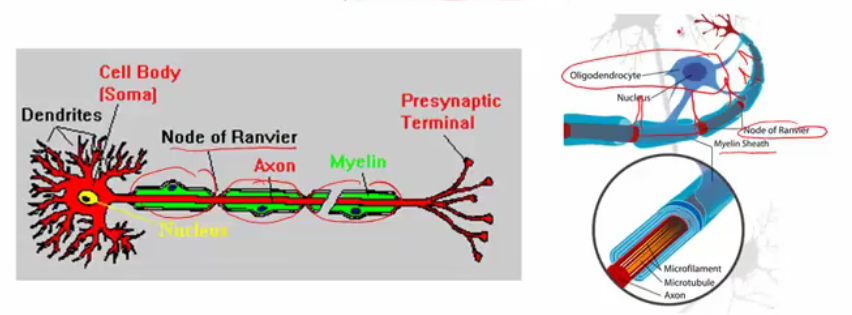
\includegraphics[width=0.7\linewidth]{./figures/myelin}
\caption{Myelination of Axons}
\label{fig:myelin}
\end{figure}



\section{Making Connections: Synapses}

A synapse is a connection or junction between 2 neurons

--- Electrical synapses use gap junctions (fast connection)

--- Chemical synapses use neurotransmitters (basic for learning and memory)

\begin{figure}[h]
\centering
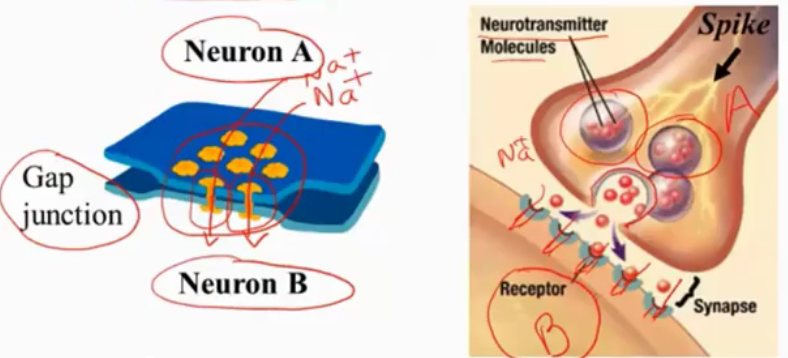
\includegraphics[width=0.7\linewidth, height=0.2\textheight]{./figures/synapse}
\caption{Synapse}
\label{fig:synapse}
\end{figure}


Synapses can be \textbf{Excitatory} or \textbf{Inhibitory}

\textbf{An Excitatory synapse:}

Input spike $\rightarrow$ Neurotransmitter release (e.g, Glutamate) $\rightarrow$ Binds to ion channel receptors $\rightarrow$ Ion channels open $\rightarrow$ Na+ influx $\rightarrow$ Depolarization due to EPSP (excitatory post-synaptic potential)

\textbf{Synapse Doctrine}

Synapses are the basic for memory and learning

\textbf{How do brain Learn? Synaptic Plasticity}: If the neuron A repeatedly takes part in firing neuron B, then the synapse form A to B is strengthened

\textbf{Long term Potentiation (LTP)}

LTP = Experimentally observed \textbf{increase} in synaptic strength that lasts for hours or days

\begin{figure}[h]
\centering
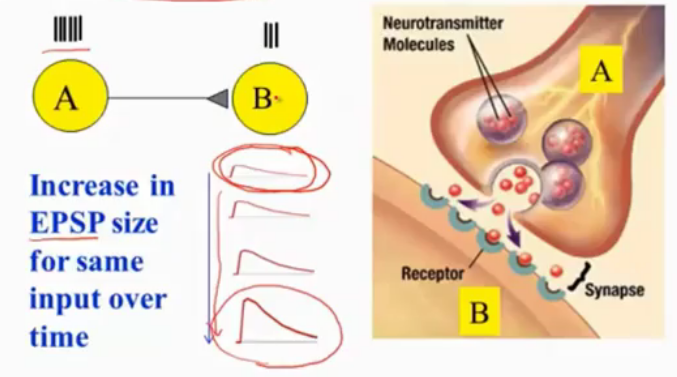
\includegraphics[width=0.7\linewidth]{./figures/LTP}
\caption{Long Term Potentiation (LTP)}
\label{fig:LTP}
\end{figure}

\textbf{Long Term Depression (LTD)}

LTD = Experimentally observed \textbf{decrease} in synaptic strength that lasts for hours or days



\textbf{Synaptic Plasticity depends on Spike Timing}

LTP/ LTD depends on relative timing of input and output spikes

\begin{figure}[h]
\centering
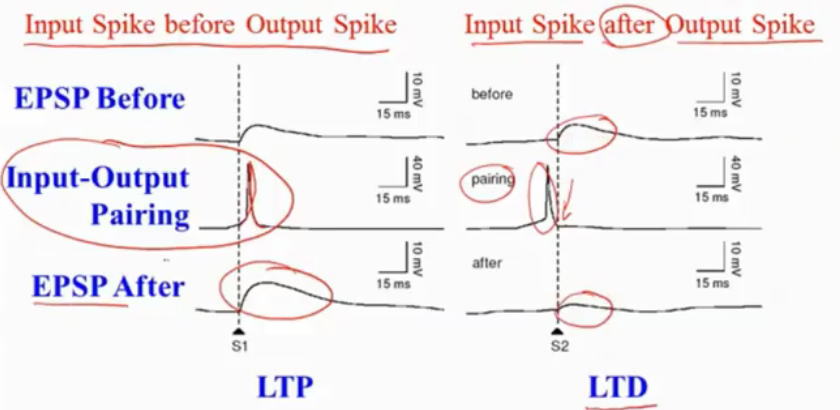
\includegraphics[width=0.7\linewidth, height=0.3\textheight]{./figures/LTP1}
\caption{relative timing of LTP and LTD}
\label{fig:LTP1}
\end{figure}

\begin{figure}[h]
\centering
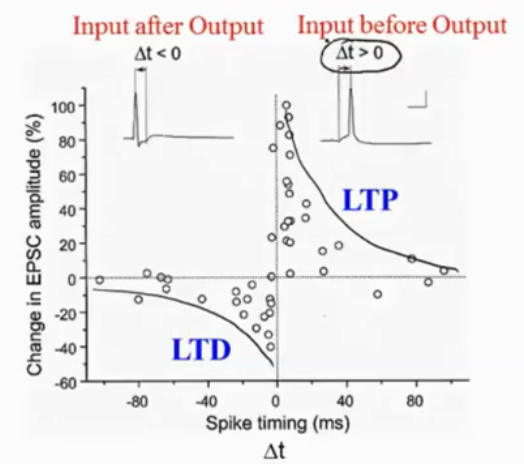
\includegraphics[width=0.7\linewidth, height=0.3\textheight]{./figures/LTPLTD2}
\caption{Spike-Timing Dependent Plasticity (STDP)}
\label{fig:LTPLTD2}
\end{figure}



\section{Time to Network: Brain Areas and Their Function}

\textbf{Organization and Function of the Nervous System}
\begin{figure}[h]
\centering
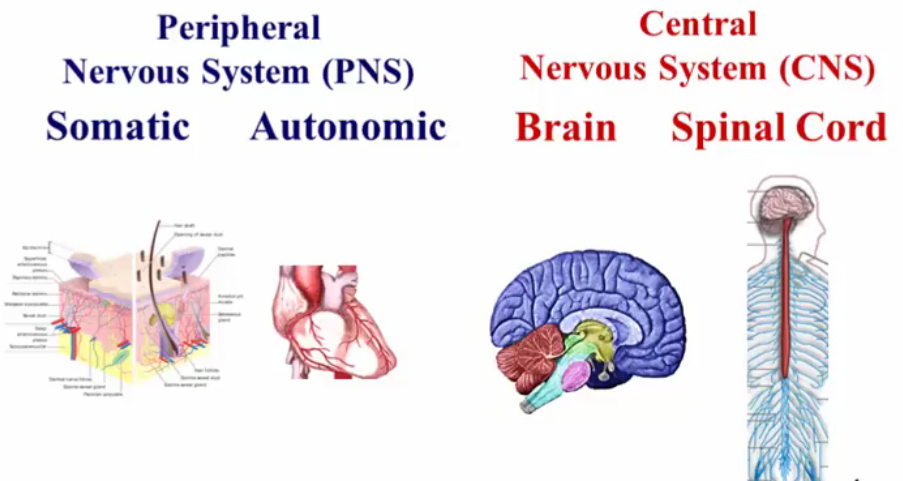
\includegraphics[width=0.7\linewidth]{./figures/nervoussystem}
\caption{Nervous System}

\label{fig:nervoussystem}
\end{figure}

 \textbf{Peripheral Nervous System(PNS)}
 
 \textbf{Somatic}: Nerves connecting to voluntary skeletal muscles and sensory receptors
 
 --- Afferent Nerve Fibers (incoming): Axons that carry info away form the periphery to the CNS
 
 --- Efferent Nerve Fibers (outgoing): Axons that carry info from the CNS outward to the periphery.
 
 \textbf{Autonomic}: Nerves that connect to the heart, blood vessels, smooth muscles
 
 \textbf{Central Nervous system (CNS)}
 
 CNS = Spinal Cord + Brain
 
 \textbf{Spinal Cord}
 
 --- Local feedback loops controls reflexes (reflex arcs)
 
 --- Descending motor control signals from the brain active spinal motor neurons
 
 --- Ascending sensory axons convey sensory information form muscles and skin back to the brain
 
 \textbf{Major Brain Regions: The Hindbrain}
 
 \begin{figure}
\centering
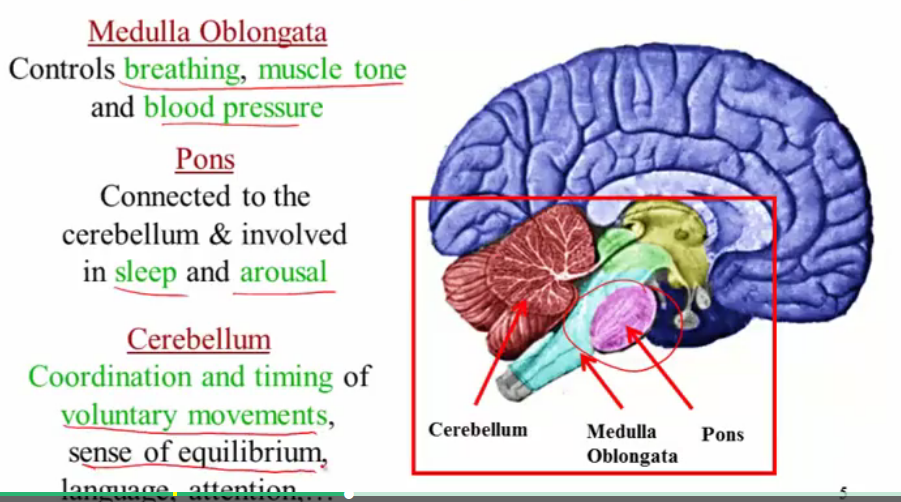
\includegraphics[width=0.7\linewidth]{./figures/hindbrain}
\caption{Hindbrain}
\label{fig:hindbrain}
\end{figure}

\textbf{Major Brain Regions: Midbrain and Retic. Formation}

\textbf{Midbrain}: Eye movements, visual and auditory reflexes

\textbf{Reticular Formation}: Modulates muscle reflexes, breathing and pain perception. Also regulates sleep, wakefulness and arousal

\begin{figure}[h]
\centering
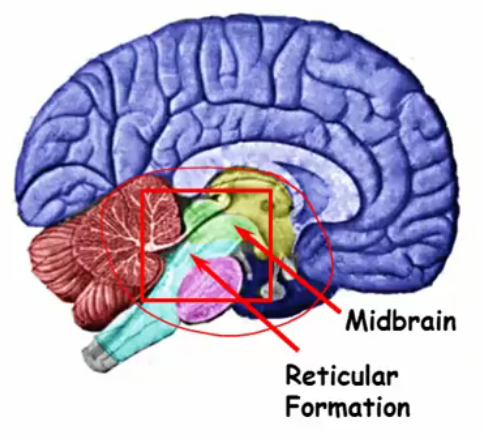
\includegraphics[width=0.7\linewidth]{./figures/midbrain}
\caption{Midbrain and Retic. Formation}
\label{fig:midbrain}
\end{figure}

\textbf{Major Brain Regions: Thalamus and Hypothalamus}

\textbf{Thalamus}: Relay station for all sensory info (except smell) to the cortex, regulates sleep/wakefulness

\textbf{Hypothalamus}: Regulates basic needs: Fighting, Fleeing, Feeding and Mating

\begin{figure}[h]
\centering
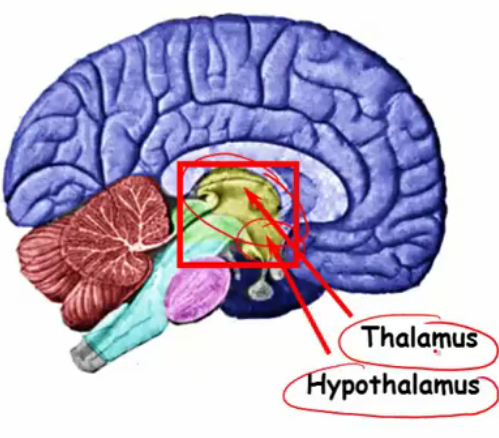
\includegraphics[width=0.7\linewidth]{./figures/Thalamus}
\caption{Thalamus and Hypothalamus}
\label{fig:Thalamus}
\end{figure}

 
\textbf{Major Brain Region: THe Cerebrum}

Consists of: Cerebral cortex, basal ganglia, hippocampus, and amygdala

Involved in perception and motor control, cognitive functions, emotion, memory, and learning

\begin{figure}[h]
\centering
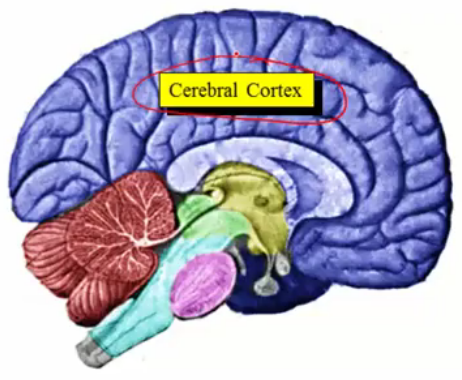
\includegraphics[width=0.7\linewidth]{./figures/cerebrum}
\caption{Cerebrum}
\label{fig:cerebrum}
\end{figure}


\textbf{Cerebral Cortex}: A layered Sheet of Neurons

Convoluted surface of cerebrum, about 1/8 of an inch thick

Six layers of neurons

\begin{figure}[h]
\centering
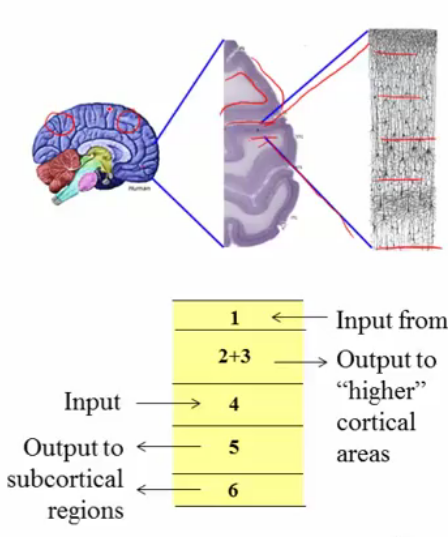
\includegraphics[width=0.7\linewidth]{./figures/cerabral}
\caption{Cerebral Cortex}
\label{fig:cerabral}
\end{figure}

\pagebreak

 
\end{document}